\documentclass[a4paper,14pt]{article}
\usepackage[14pt]{extsizes}




\usepackage{cmap}					% поиск в PDF
\usepackage{mathtext} 				% русские буквы в формулах
\usepackage[T2A]{fontenc}			% кодировка
\usepackage[utf8]{inputenc}			% кодировка исходного текста
\usepackage[english,russian]{babel}	% локализация и переносы
\usepackage{ulem}                   % зачеркнутый текст
\usepackage{amssymb}			% пакет математики
\usepackage{float}
\usepackage{amsmath}
\usepackage{graphicx}
\DeclareGraphicsExtensions{.png}

%%% Страница
%\usepackage{extsizes} % Возможность сделать 14-й шрифт
\usepackage[left=1cm,right=1cm,top=1cm,bottom=1cm]{geometry} % Простой способ задавать поля
\pagestyle{empty}

\begin{document}


\begin{center}
ФЕДЕРАЛЬНОЕ ГОСУДАРСТВЕННОЕ ОБРАЗОВАТЕЛЬНОЕ БЮДЖЕТНОЕ УЧРЕЖДЕНИЕ ВЫСШЕГО ОБРАЗОВАНИЯ

    \textbf{«ФИНАНСОВЫЙ УНИВЕРСИТЕТ ПРИ ПРАВИТЕЛЬСТВЕ РОССИЙСКОЙ ФЕДЕРАЦИИ»}

Факультет информационных технологий и анализа больших данных

Департамент анализа данных и машинного обучения

\textit{
	\textbf{Дисциплина: «Теория вероятностей и математическая статистика»}}

\textit{Направление подготовки: 01.03.02 «Прикладная математика и информатика»}

\textit{Профиль: «Анализ данных и принятие решений в экономике и финансах»}

\textit{Форма обучения очная, учебный 2020/2021 год, 4 семестр}

\textbf{Билет 125}

\end{center}

\begin{enumerate}


\item


Сформулируйте определение случайной выборки из конечной генеральной совокупности. Какие
виды выборок вам известны? Перечислите (с указанием формул) основные характеристики выборочной и генеральной совокупностей




Здесь очень много исчерпывающей информации о выборках из генеральной совокупности и про различные виды выборок


\item



Случайные величины $X$ и $Y$ независимы и имеют равномерное
распределение на отрезках $[0;7]$ и $[0;3]$ соответственно. Для случайной величины $Z=\frac{Y}{X}$ найдите: 
1) функцию распределения $F_Z(x)$;
2) плотность распределения $f_Z(x)$ и постройте график плотности;
3) вероятность $\P(0,\!006\leqslant Z\leqslant 0,\!519)$.




%\folder 2_53d18.png
1) Функция распределения $F_Z(x)$ имеет вид:
$
F_Z(x)=\left\{
\begin{array}{l}
0, x\leqslant 0;\\
\frac{7 x}{6}, 0\leqslant x\leqslant \frac{3}{7}\approx 0,\!429;\\
1 - \frac{3}{14 x}, x\geqslant\frac{3}{7};
\end{array}.
\right.
$
2) Плотность распределения $f_Z(x)$ имеет вид:
$
f_Z(x)=\left\{
\begin{array}{l}
0, x<0;\\
\frac{7}{6}, 0\leqslant x\leqslant \frac{3}{7}\approx 0,\!429;\\
\frac{3}{14 x^{2}}, x\geqslant\frac{3}{7};
\end{array}.
\right.
$


\begin{figure}[H]
    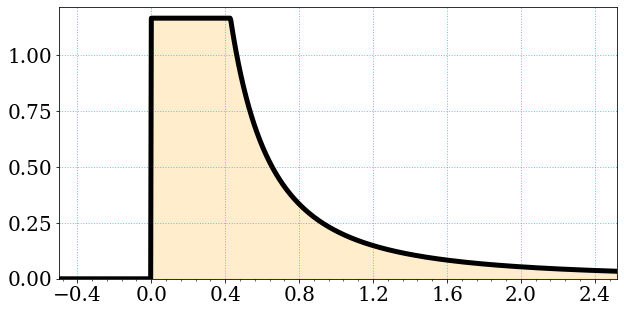
\includegraphics[width=0.9\textwidth]{2_53d18}
\end{figure}


3) вероятность равна:
$
\P(0,\!006\leqslant Z\leqslant 0,\!519)=
0,\!57962.
$


\item


(10) Известно, что доля возвратов по кредитам в банке имеет распределение $F(x) = x ^{\beta}, 0 \leqslant x \leqslant 1$.
Наблюдения показали, что в среднем она составляет $87,5\%$. Методом моментов оцените параметр $\beta$ и
вероятность того, что она опуститься ниже $53\%$




Найдём плотность рапределения как интеграл от ФР, а дальше всё и вовсе простою Ответ: $1174711139837$


\item


(10) В группе $\Omega$ учатся студенты:$\omega _{1}...\omega _{25}$ . Пусть $X$ и $Y$ – 100-балльные экзаменационные оценки по
математическому анализу и теории вероятностей. Оценки $\omega _{i}$ студента обозначаются: $x _{i} = X(\omega _{i})$ и $y _{i} = Y(\omega _{i})$, $i = 1...25$. Все оценки известны
$x _{0} = 73, y _{0} = 44$, $x _{1} = 44, y _{1} = 83$, $x _{2} = 49, y _{2} = 41$, $x _{3} = 36, y _{3} = 32$, $x _{4} = 48, y _{4} = 60$, $x _{5} = 53, y _{5} = 37$, $x _{6} = 70, y _{6} = 86$, $x _{7} = 61, y _{7} = 82$, $x _{8} = 42, y _{8} = 57$, $x _{9} = 94, y _{9} = 40$, $x _{10} = 44, y _{10} = 78$, $x _{11} = 85, y _{11} = 78$, $x _{12} = 48, y _{12} = 66$, $x _{13} = 88, y _{13} = 82$, $x _{14} = 31, y _{14} = 39$, $x _{15} = 84, y _{15} = 68$, $x _{16} = 49, y _{16} = 51$, $x _{17} = 84, y _{17} = 55$, $x _{18} = 65, y _{18} = 67$, $x _{19} = 37, y _{19} = 99$, $x _{20} = 46, y _{20} = 31$, $x _{21} = 84, y _{21} = 46$, $x _{22} = 40, y _{22} = 67$, $x _{23} = 86, y _{23} = 54$, $x _{24} = 89, y _{24} = 32$
Требуется
найти следующие условные эмпирические характеристики: 1) ковариацию $X$ и $Y$ при условии, что одновременно $X \geqslant 50$
 и $Y \geqslant 50$; 2) коэффициент корреляции $X$ и $Y$ при том же условии.




1) Ковариация = $-345.5$
2) Коэффициент корреляции = $-2.9554$


\item


(10) Эмпирическое распределение признаков $X$ и $Y$ на генеральной совокупности $\Omega$ задано таблицей частот  
 
\begin{tabular}{ | c | c | c | c | }
\hline
 & $Y = 2$ & $Y = 4$ & $Y = 5$  \\ \hline
$X = 200$ & $16$ & $19$ & $5$\\ \hline
$X = 300$ & $25$ & $10$ & $25$\\
\hline
\end{tabular}

Из $\Omega$ случайным образом без возвращения извлекаются $6$ элементов. 
Пусть $\bar X$ и $\bar Y$ – средние значения признаков на выбранных элементах. 
Требуется найти: 1) математическое ожидание $\mathbb{E}(\bar Y)$; 2) стандартное отклонение $\sigma(\bar X)$ ; 
3) ковариацию $Cov(\bar X, \bar Y)$




1) математическое ожидание $\mathbb{E}(\bar Y)$: $3.48$ 
2) стандартное отклонение $\sigma(\bar X)$: $256.5595$
3) ковариацию $Cov(\bar X, \bar Y)$: $0.5887$


\item


(10) Пусть $X _{1}$, $X _{2}$, $X _{3}$, $X _{4}$ выборка из $N(\theta, \sigma ^{2})$. Рассмотрим две оценки параметра $\theta$:
\[\hat \theta _{1} = \frac{3X _{1} + X _{2} + 4X _{3} + 2X _{4}}{10}, \hat \theta _{1} = \frac{X _{1} + 6X _{2} + 2X _{3} + X _{4}}{10}\]
a) Покажите, что обе оценки несмещенные.
б) Какая из оценок оптимальная?




Обе они несмещенные, потому что в числителе выходит в сумме 10.
Какая-то точно должна быть, а может и нет....


\end{enumerate}

\begin{figure}[H]
	Подготовил
	\hfill
	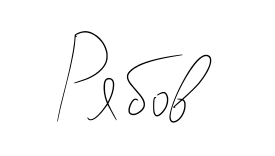
\includegraphics[width=2cm]{Prepared}
	П.Е. Рябов
\end{figure}


\begin{figure}[H]
	Утверждаю:\\
	Первый заместитель\\
	руководителя департамента\\
	Дата 01.06.2021
	\hfill
	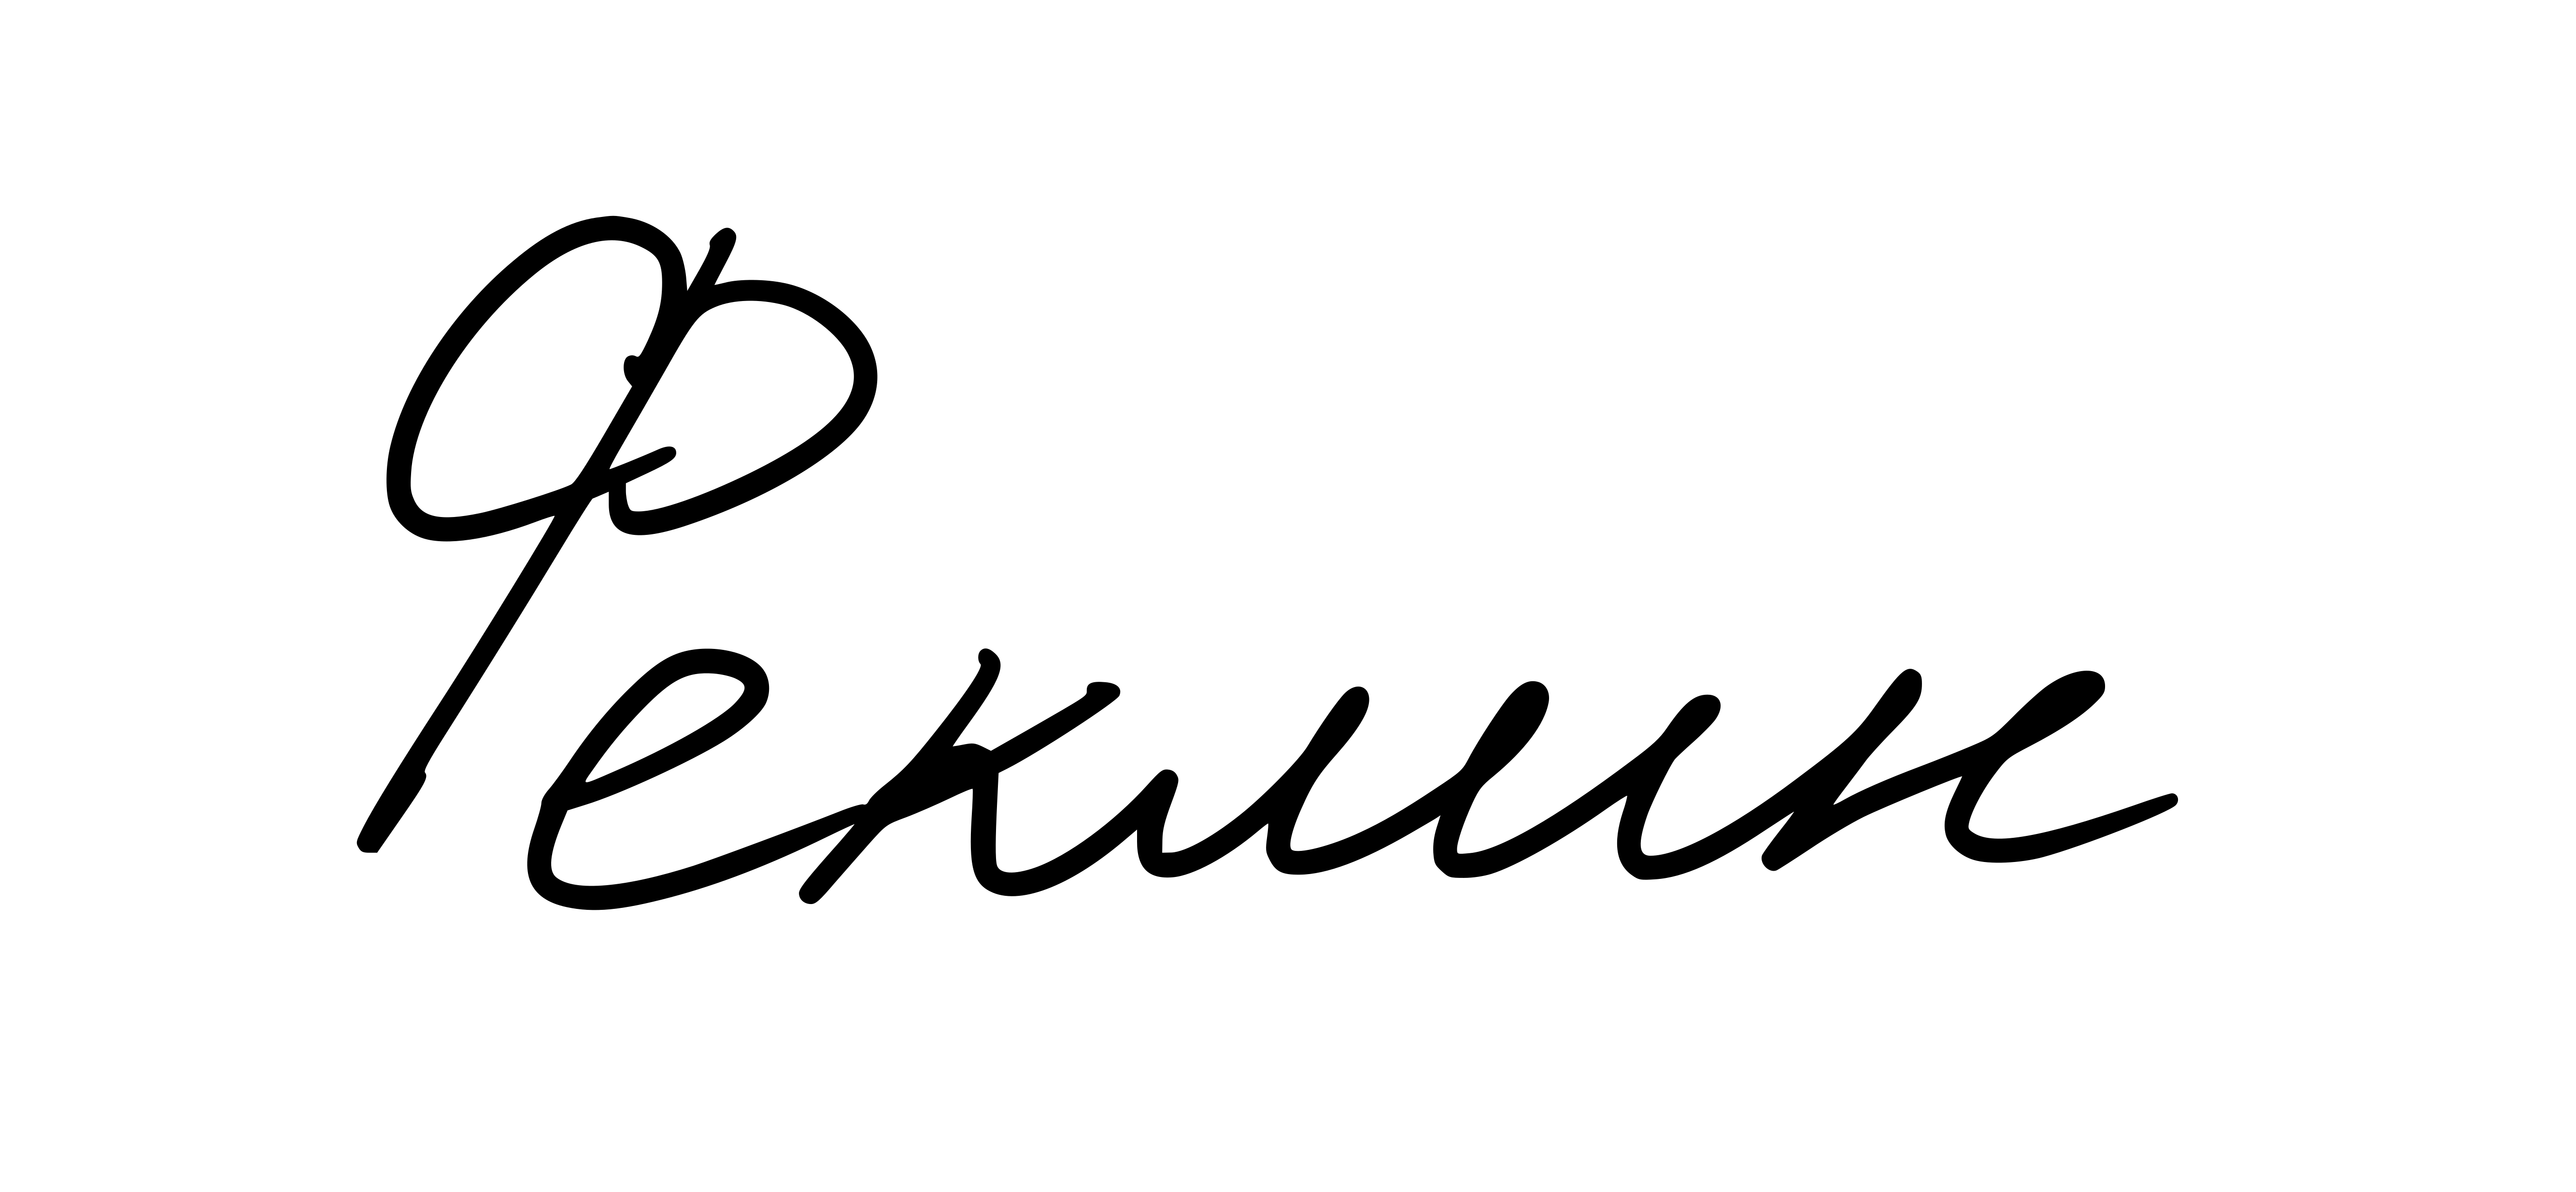
\includegraphics[width=2cm]{Approved}
	Феклин В.Г.
\end{figure}

\end{document}

